\section{Methods}
\label{sec:methods}
%In response to stakeholder and public preferences, forest planners often manage forests for multiple ecosystem services simultaneously, such as wildlife habitat, recreation, goods production, aesthetics, and carbon sequestration. Due to conflicts among these ecosystem services, however, often forest planners cannot simultaneously maximize the provision of all of them. Instead, the provision of some services must be reduced to increase achievement in others. In these cases, the goal is to find the best compromise alternatives.
%
%It is currently unknown how climate change will alter the trade-off relationships among bundled ecosystem services. This drives uncertainty in whether and how forest planners must change their compromise strategies to maintain a desired balance among ecosystem services. In this section, I describe a case study in the Deschutes National Forest in which I used multi-objective optimization to quantify the changes in trade-off relationships, comparing the results under three different climate change scenarios.
%

Bundled ecosystem services conflict with one another, and I argue that understanding the change in this conflict over time will enable forest planners to make more informed management decisions. Here, I provide formal definitions of what it means for ecosystem services to conflict, how to measure changes in conflict, and how a change in conflict impacts trade-off relationships.

\subsection{Terminology}
To aid in the discussion of conflict and trade-offs, prior to defining the new conflict metric, I first present the definitions and notation used here. Note that in the following, superscripts generally refer to solution identifiers and subscripts generally refer to dimension identifiers. For example, $\mathbf{x}^1$ refers to the first solution while $x^1_i$ refers to the $i$-th dimension of the first solution.

\label{subsec:terminology}
\paragraph{The multi-objective problem}
Consider the $M$-objective optimization problem
\begin{align}
\text{Maximize}& \notag \\
& \mathbf{f} = [f_1(\mathbf{x}), f_2(\mathbf{x}), \ldots, f_M(\mathbf{x}) ]^T \label{eqn:generalObj}\\
\text{subject to}& \notag \\
& \mathbf{x} \in X \label{eqn:generalConstraint}
\end{align}
with \textit{objective functions} $f_i(\mathbf{x}), i \in \{1,\ldots,M\}$ and feasible \textit{decision vectors} (or \textit{solutions}) $\mathbf{x} \in \mathbb{R}^n$ where $n$ is the number of decision variables in the optimization problem. A set of equality and inequality constraints determine the \textit{feasible decision space} $X$. Each objective function $f_i : \mathbb{R}^n \mapsto \mathbb{R}$ maps decision vectors to scalars in $\mathbb{R}$. The vector objective function $\mathbf{f} : X \mapsto \mathbb{R}^M$ maps the feasible decision space to the \textit{objective space} $\mathbb{R}^M$. The set of all objective functions is the \textit{objective set} $\mathcal{M} = \{f_1,\ldots,f_M\}$.

\paragraph{Dominance and frontiers}
A solution $\mathbf{x}^1$ is said to \textit{dominate} another solution $\mathbf{x}^2$ ($\mathbf{x}^1 \succ \mathbf{x}^2$) if
\begin{align}
\forall f_i \in \mathcal{M} \; f_i(\mathbf{x}^1) \ge f_i(\mathbf{x}^2) \text{ and } \exists f_i \in \mathcal{M} : f_i(\mathbf{x}^1) > f_i(\mathbf{x}^2)
\end{align}
The set of non-dominated solutions to the multi-objective problem \eqref{eqn:generalObj} and \eqref{eqn:generalConstraint} is referred to as the \textit{Pareto-optimal set} $P = \{\mathbf{x} \in X | \nexists \mathbf{y} \in X : \mathbf{y} \succ \mathbf{x} \}$.

The \textit{Pareto-optimal frontier}, the \textit{efficient frontier} or, simply, the \textit{frontier} $Z$ is the corresponding set of $M$-dimensional \textit{objective vectors} $\mathbf{z} = [f_1(\mathbf{x}),f_2(\mathbf{x}),\ldots,f_M(\mathbf{x})]$. That is,
\begin{align}
Z = \{\mathbf{z} = [f_1(\mathbf{x}),\ldots,f_M(\mathbf{x})] \:|\: \mathbf{x} \in P\}
\end{align}
Objective vectors' components are referred to in subscripts:
\begin{align}
\mathbf{z} = [z_1, z_2, \ldots, z_M]
\end{align}

\paragraph{Ideal and nadir objective vectors}
The \textit{ideal objective vector} is defined as the vector
\begin{align}
\mathbf{z}^{\text{ideal}} = \max_{\mathbf{x} \in X}\{f_i(\mathbf{x})\} \quad \forall i \in \mathcal{M}.
\end{align}
Analogously, define the nadir solution as the vector
\begin{align}
\mathbf{z}^{\text{nadir}} = \min_{\mathbf{x} \in X}\{f_i(\mathbf{x})\} \quad \forall i \in \mathcal{M}.
\end{align}


\paragraph{Sub-dimensions} Define the \textit{sub-dimensional objective set} $\mathcal{L} \subset \mathcal{M}$ as a subset of the objective functions $f_i \in \mathcal{M}$. Call the cardinality of this set $L$. The \textit{sub-dimensional objective vector} (specifically, the $L$-dimensional objective vector) for the solution $\mathbf{x}^i$ is the vector denoted $\mathbf{z}^i_\mathcal{L}$ whose components are $z^i_\ell = f_\ell(\mathbf{x}^i)$, $\forall \ell \in \mathcal{L}$. That is, they are the components of $\mathbf{z}^i$ that correspond to the objectives in $\mathcal{L}$.

\paragraph{Trade-offs}
The \textit{trade-off} between two objective vectors $\mathbf{z}^1$ and $\mathbf{z}^2$ is the vector of differences in their objective achievements:
\begin{align}
\mathbf{\tau}^{1,2} = [z^2_1 - z^1_1, z^2_2 - z^1_2, \ldots, z^2_M - z^1_M]
\end{align}
Note that $\mathbf{\tau}^{1,2} = - \mathbf{\tau}^{2,1}$.

Given a sub-dimensional objective set $\mathcal{L}$, define the \textit{sub-dimensional trade-off} $\tau^{1,^2}_\mathcal{L}$ as the vector with components $\tau^{1,2}_\ell$, $\forall \ell \in \mathcal{L}$.

\paragraph{Conflict, monotonicity, bundles and stacks}
Objectives in an objective set $\mathcal{L}$ \textit{do not conflict} if the objectives improve simultaneously:
$\forall \mathbf{z}^1, \mathbf{z}^2 \in Z, i \in \mathcal{L}$
\begin{align}
(z^1_i \ge z^2_i) \Rightarrow (z^1_j \ge z^2_j) \quad \forall j \in \mathcal{L}, j \neq i \label{eqn:objPairHarmony}
\end{align}
If \eqref{eqn:objPairHarmony} does not hold, then the objectives conflict. Any pair of objectives $i,j \in \mathcal{M}$ such that equation \eqref{eqn:objPairHarmony} holds are said to \textit{increase monotonically}. If 
\begin{align}
(z^1_i \ge z^2_i) \Rightarrow (z^1_j \le z^2_j) \quad \forall \mathbf{z}^1, \mathbf{z}^2 \in Z, j \neq i \label{eqn:objPairMonoDec}
\end{align}
holds, then the objectives are said to \textit{decrease monotonically}. When the objectives represent goods or services, a set of objectives that conflict is defined as a \textit{bundle} and a set of objectives that do not conflict is defined as a \textit{stack}.

The means of detecting conflict among an objective set (equation \eqref{eqn:objPairHarmony})is functionally equivalent to that used by other studies, such as Brockhoff and Zitzler (2009) \cite{brockhoff2009objective} and Purshouse and Fleming (2003) \cite{purshouse2003conflict}.

\subsection{A new measure of conflict}
After determining that objectives conflict with one another (see equation \eqref{eqn:objPairHarmony}), one may wish to determine the severity of the conflict. Consider the frontiers in Figure \ref{fig:ConflictVariesExample}. The conflict between maximization objectives $i$ and $j$ is greatest in Frontier C and least in Frontier A.
\begin{figure}[ht]
\centering

\includegraphics[width=.6\textwidth]{../images/ConflictVariesExample}
\caption[Example of varying conflict between objectives]{Varying conflict between objectives. The conflict between maximization objectives $i$ and $j$ increases from Frontier A to Frontier B to Frontier C.}
\label{fig:ConflictVariesExample}
\end{figure}

Many authors have previously measured conflict between objectives \cite{brockhoff2009objective}\cite{purshouse2003conflict}\cite{gal1977redundant}, with most commonly used metrics deriving from measures of linear correlation (such as the Pearson correlation coefficient \cite{deb2006searching}) or rank correlation (such as Kendall's Tau \cite{kanoulas2009empirical} or Spearman's rho \cite{karande2012application}%, and Zitzler's $\delta$-error \cite{brockhoff2006all}).
). The intended use of these metrics is often the removal of redundant objectives from a many-objective optimization problem. In such cases, measures of monotonicity or correlation alone are adequate. However, for a more nuanced understanding of the relationship between the objectives, a different metric is required.

Let $\mathbf{z}_{ij}$ be the sub-dimensional objective vector comprised of only the components corresponding to the $i$th and $j$th objectives $\mathbf{z}_{ij} = [z_i,z_j]$. I define the following measure of conflict between objectives $i$ and $j$:
\begin{align}
C_{ij} = \frac{(1-\rho_{ij})\overbar{d}_{ij}}{2 d_{\max,ij}} \label{eqn:defConflict}
\end{align}
where $\overbar{d}_{ij}$ is the average sub-dimensional distance from objective vectors to the ideal solution:
\begin{align}
\overbar{d}_{ij} = \frac{1}{|Z|} \sum_{\mathbf{z} \in Z} ||\mathbf{z}^{\text{ideal}}_{ij} - \mathbf{z}_{ij}||
\end{align}
and
\begin{align}
d_{\max,ij} = ||\mathbf{z}^{\text{ideal}}_{ij} - \mathbf{z}^{\text{nadir}}_{ij}||
\end{align}
and $\rho_{ij}$ is Spearman's rank-correlation coefficient for the solutions' achievements in objectives $i$ and $j$. Note that $C_{ij} \in [0,1)$, taking smaller values when there is less conflict between objectives $i$ and $j$ and larger values when there is more.

The conflict metric proposed here (equation \eqref{eqn:defConflict}) addresses two major issues:
\begin{enumerate}
\item \textbf{Indifference to non-conflicting relationships}. Per the definition of conflict in equation \eqref{eqn:objPairHarmony}, objectives $i,j$ that increase monotonically are not in conflict. Accordingly, $C_{ij}$ should equal 0 in all such cases. This is true for the new metric, since for monotonically increasing objectives $1-\rho_{ij} = 0$.
\item \textbf{Consideration of objective achievement}. Recall Figure \ref{fig:ConflictVariesExample} and the intuitive notion that the conflict between objectives $i$ and $j$ is stronger in Frontier C than it is in Frontier B than it is in Frontier A. This notion is guided by the idea that the closer objective vectors are to the sub-dimensional ideal solution on average, the less the conflict between the objectives. That is, that greater simultaneous objective provision is indicative of less conflict. The proposed metric accounts for this, while correlation measures do not. In the extreme case of monotonically decreasing objectives, $\frac{(1-\rho_{ij})}{2} = 1$, so $C_{ij} = \frac{\overbar{d}{ij}}{d_{\max,ij}}$. See Figure \ref{fig:WhyOursIsBetter} for an example.
\end{enumerate}
\begin{figure}[ht]
\centering

\includegraphics[width=.9\textwidth]{../images/WhyOursIsBetter}
\caption[Comparing the proposed conflict metric to others used in multi-objective optimization]{Comparing the proposed metric for conflict $C_{ij}$ against the Pearson product-moment and the Spearman rank correlation coefficients ($\rho_{ij}$ and $\rho_{s,ij}$, respectively). While the latter two are identical for frontiers A and C, the proposed metric is greater for frontier C than it is for A. This is because it accounts for the average relative distance to the sub-dimensional ideal objective vector.}
\label{fig:WhyOursIsBetter}
\end{figure}

\subsection{Study system}
\label{subsec:studyArea}
To quantify the impacts of climate change on the relationships among and the joint provision of bundled forest ecosystem services, I employ multi-objective optimization on a study system in the Deschutes National Forest known as the Drink Planning Area. The Drink Area is a 7056 ha area on the east slopes of the Cascade Mountain Range (see Figure \ref{fig:drinkOverview}). Like many forests, the Drink is managed for the simultaneous provision of multiple ecosystem services.  The ecosystem services were selected through a process involving stakeholder meetings and discussions regarding compatible ecosystem services. For the current work, a subset of the chosen ecosystem services was selected for study. While the USFS manages for many services simultaneously, many of the services are ``stacked'' rather than bundled, meaning that the ecosystem services are not in conflict. That is, maximizing the provision of one ecosystem service simultaneously maximizes another. Stacked ecosystem services need not all be studied with multi-objective optimization, since the selection and maximization of one ecosystem service entails the maximization of all in the stack. For that reason, we disregard non-conflicting ecosystem services and select a minimal bundle on which to employ multi-objective optimization. Those that do not conflict can be stacked post-optimization.

The minimal bundle selected for this case study is a set of three ecosystem services. The Forest Service seeks to ensure their sustained provision, and this may require an understanding of how these ecosystem services are impacted, jointly and independently, by climate change.

\begin{figure}[ht]
\centering
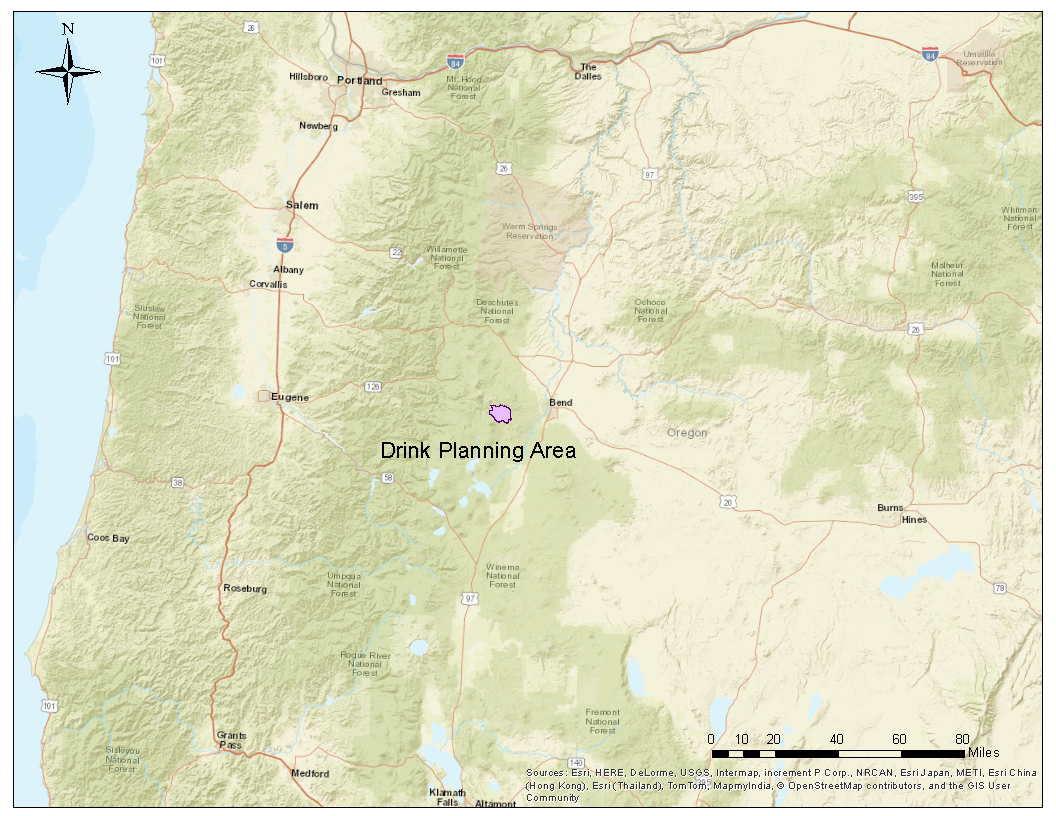
\includegraphics[width=.85\textwidth]{../images/DrinkMap_Overview}
\caption[Overview of the study system, the Drink Planning Area]{Overview of the study system, the Drink Planning Area (in purple), consisting of 7056 ha in the Deschutes National Forest.}
\label{fig:drinkOverview}
\end{figure}

The first of these ecosystem services is the provision of habitat for the northern spotted owl (NSO) (\textit{Strix occidentalis caurina}). The NSO is a common, if controversial, indicator species in Pacific Northwest forests. Because of the availability of dense old growth forest in the Drink, approximately 43\% of the area serves as habitat for the NSO (see Figure \ref{fig:drinkOwlAndWatershed}). The USFS is required to protect this species as it is listed as threatened and therefore protected by the Endangered Species Act of 1973 \cite{congress1973endangered}.

The second ecosystem service the USFS seeks to provide is protection from high severity wildfire. This protection is achieved by way of silvicultural treatments applied to designated treatment areas (forest stands) across the Drink. The types of treatments assigned are defined in the appendix, \S \ref{chap:appBTreatmentSpec}. The efficacy of these treatments is measured by comparing the fire hazard rating of the stand before and after treatment. The fire hazard rating is described in more detail later and is summarized in Table \ref{tab:firehazards}. Implementing the silvicultural treatments to reduce the fire hazard rating of the Drink is critical not only because it protects the habitat of the NSO, but also because the Drink Area houses the municipal watershed for the cities of Bend, OR and Sisters, OR (see Figure \ref{fig:drinkOwlAndWatershed}). Wildfires pose a threat to these cities' water supply, because wildfires can cause soil water repellency, surface runoff, and debris torrents \cite{ice2004effects} which would degrade the quality of the watershed. In addition, the Drink has never before undergone fuels treatments, which increases the expected severity of a fire should one occur. 
\begin{figure}
\centering
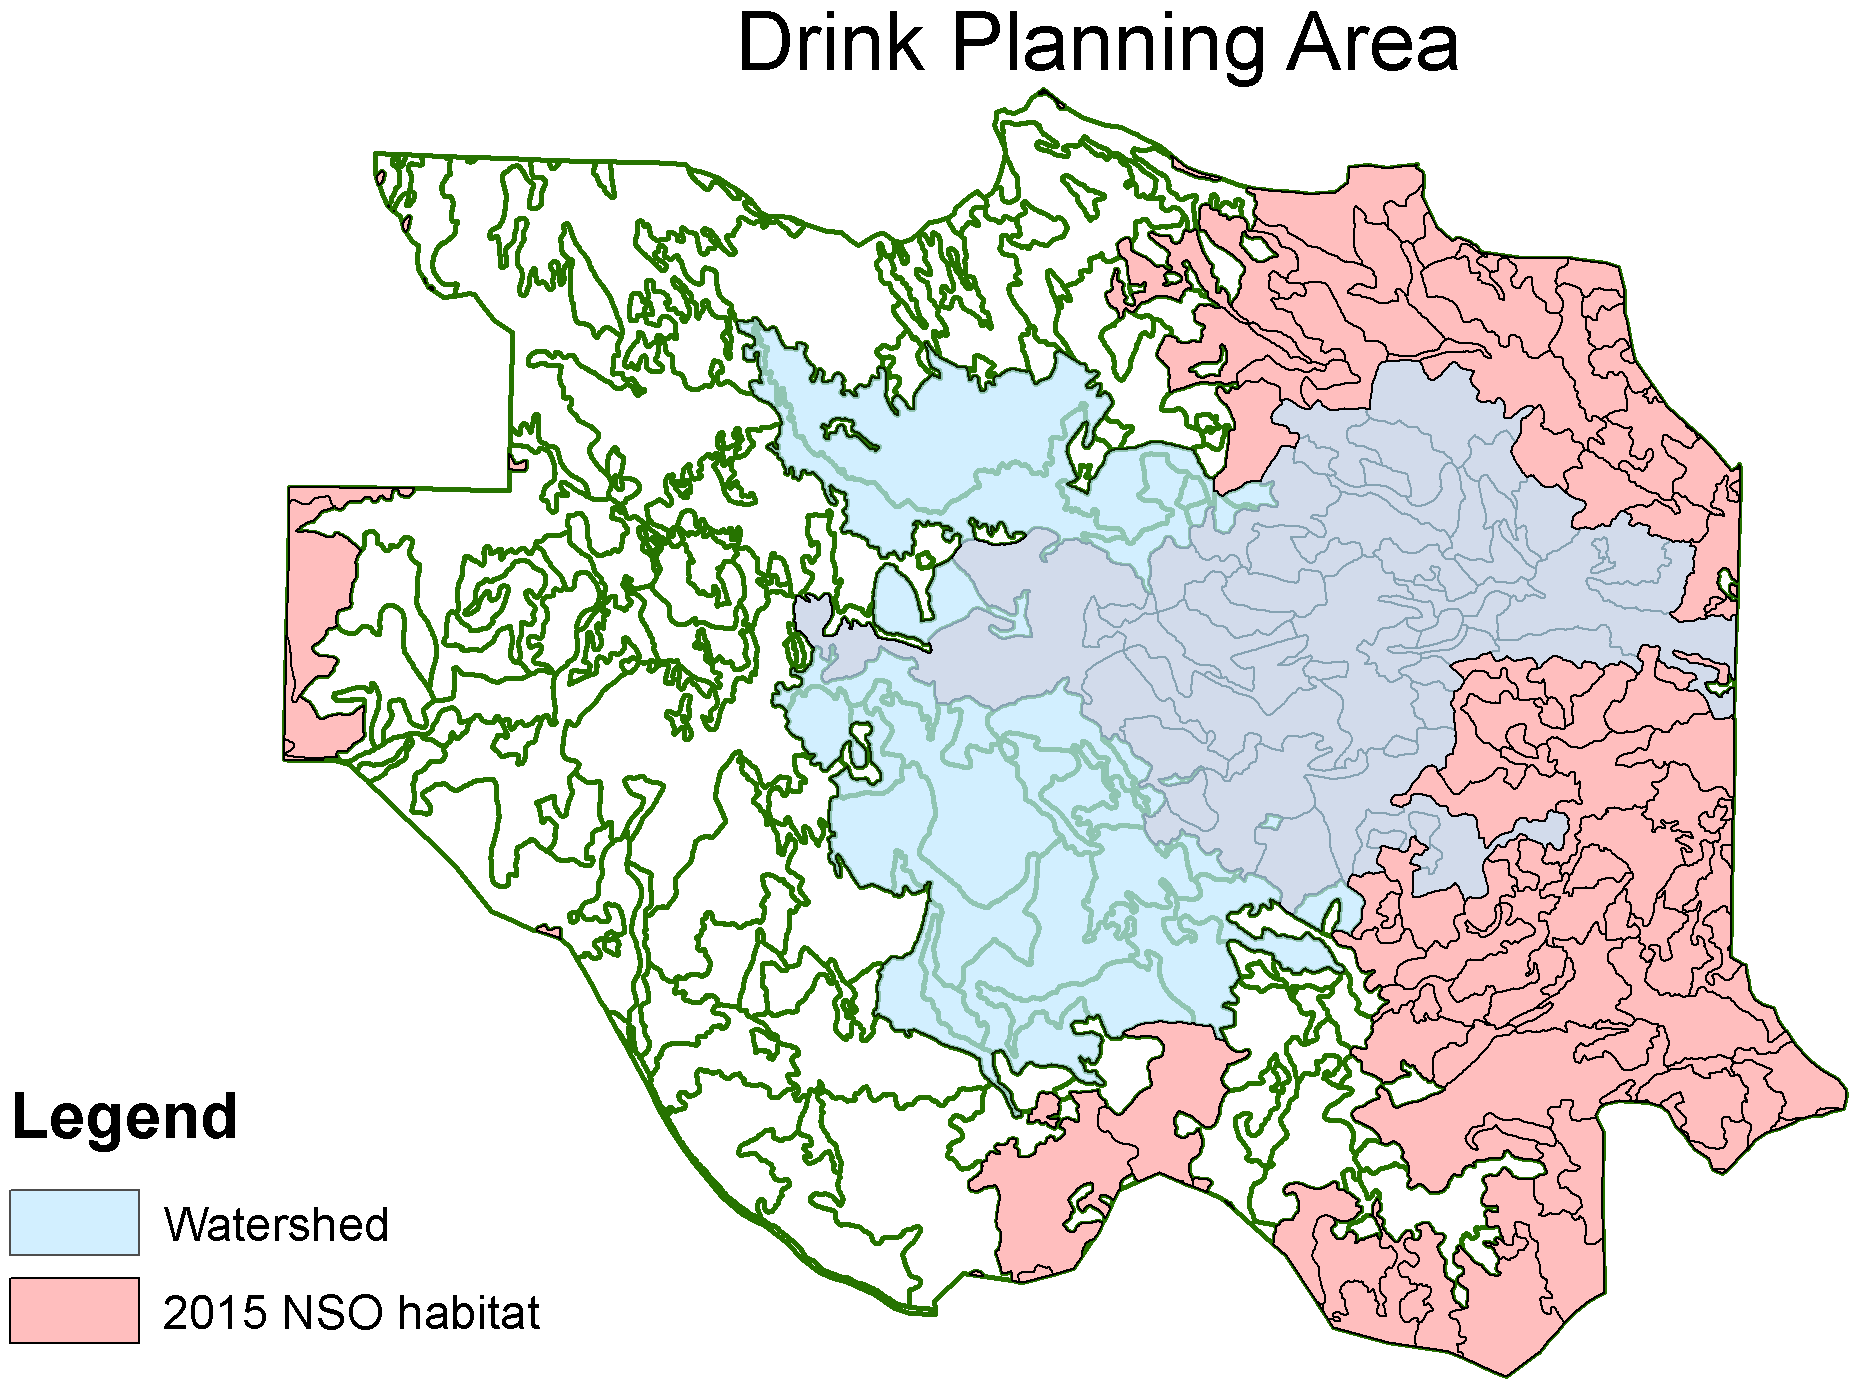
\includegraphics[width=.5\textwidth]{../images/DrinkMap_NSOAndWatershed}
\caption[NSO Habitat and municipal watershed in the Drink Planning Area]{Location of the municipal watershed and the suitable NSO habitat in the Drink area at the beginning of the planning horizon (2015). Interior polygons are the 303 management units.}
\label{fig:drinkOwlAndWatershed}
\end{figure}

Finally, the Forest Service seeks to provide a watershed with minimal sediment content. While the silvicultural treatments intend to provide long-term protection of the watershed, the implementation of the treatments has the potential to introduce short-term increases in sediment delivery \cite{o2005conceptual}. This is expected to be especially true in the Drink Area, where local Forest Service staff have noted that the watershed is unusually susceptible to spikes in sediment delivery as a result of foot traffic and activities that occur within the watershed.

The changing climate will likely impact the provision of these ecosystem services and their relationships with one another. The extent of these changes will depend on the severity of the realized climate change. Thus, to understand the potential impacts, multiple climate change scenarios representing a range of severities must be considered. The following section describes the climate scenarios considered in this case study.

\subsection{Climate Scenarios Considered}
In their assessments on the changing climate, the Intergovernmental Panel on Climate Change (IPCC) uses a scenario-based approach, considering many models of future climates from research groups around the world. They make no attempt to predict which of the future climates is most likely or to quantify the probability of realization of any one scenario. This same scenario-based approach is employed here in studying the potential impacts of climate change on trade-off relationships among bundled ecosystem services.

Here, the alternative future climates considered are climate scenarios from the first working group (WG1) of the IPCC's Fifth Assessment (AR5) \cite{ipcc2013climate}. Given the large number of potential future climates considered by the IPCC (see the list of experiments considered in AR5 \cite{ipccListOfAR5Models}) combined with the computational complexity involved in the study of each one, I selected a subset of three future climate scenarios for this analysis. Hereafter the scenarios are referred to as ``None'', ``Ensemble RCP 4.5'', and ``Ensemble RCP 8.5''.

The first scenario, ``None'', is the assumption of no climate change. While the number of studies incorporating climate change is increasing, this is still the assumption used for many modern studies such as Schroder (2013) \cite{schroder2016multi}, from which this study is derived. Because it has served as the basis for many studies and assumes a static climate resembling today's, the ``None'' climate scenario serves as a control against which to compare the other two future climate scenarios.

As their names suggest, the second and third scenarios are ensembles. Each ensemble is an assembly of 17 global circulation models (GCMs) used in IPCC AR5. The selection of component GCMs in the ensembles was performed by the USFS's Climate-Forest Vegetation Simulator (FVS) \cite{dixon2002essential} team. The list of the 17 scenarios included in the ensemble can be found in Crookston (2016) \cite{ClimateModelsInFVSEnsemble}. Each component GCM has a corresponding climate surface which contains a vector of 35 climate parameters at over 11,000 global locations for three time periods. The climate surfaces for the ensembles were created by averaging the values of all component GCMs for each climate parameter and each time period for each location. The result is a climate surface that, while temporally sparse, is spatially robust. Such a configuration is well-suited for use in the Drink Area given the area's variance in elevation and slow vegetation growth.

The two ensembles are comprised of the same 17 GCMs, but the assumed representative concentration pathways (RCP) in the component GCMs differ. The RCP indicates the additional radiative forcing in $W/m^2$ above pre-industrial levels, with higher values of forcing indicative of more severe climate change. The GCMs in the Ensemble RCP 4.5 scenario assume 4.5 $W/m^2$ of additional radiative forcing, and the GCMs in the Ensemble RCP 8.5 scenario assume 8.5 $W/m^2$ of additional radiative forcing.

These three chosen scenarios represent a range of predicted climate change severity, from a $0 \degree C$ warming by the year 2100 under the ``None'' scenario to a $2.6-4.8 \degree C$ warming under RCP 8.5 \cite{ipcc2013climate}. Comparing the trade-off relationships among the ecosystem services under this range of climate change severities allows for the quantification of the impacts of climate.

\subsection{The Multi-objective Optimization Model}
\label{sec:model}
In order to determine trade-off relationships among ecosystem services under each climate scenario, I employ multi-objective spatial optimization. This section describes the multi-objective zero-one mathematical program to optimize the joint provision of ecosystem services in the Drink Area. The model operates over an 80-year planning horizon (2015-2095) in which it assigns silvicultural treatments to forest stands that will be performed in the first or second 20 year period (2015-2035 or 2035-2055). Determining which treatment type to apply to a stand was done \textit{a priori} and is entirely dependent on silvicultural characteristics; the rules governing this assignment of treatment type can be found in the appendix, \S \ref{chap:appBTreatmentSpec}.

\begin{figure}
\centering
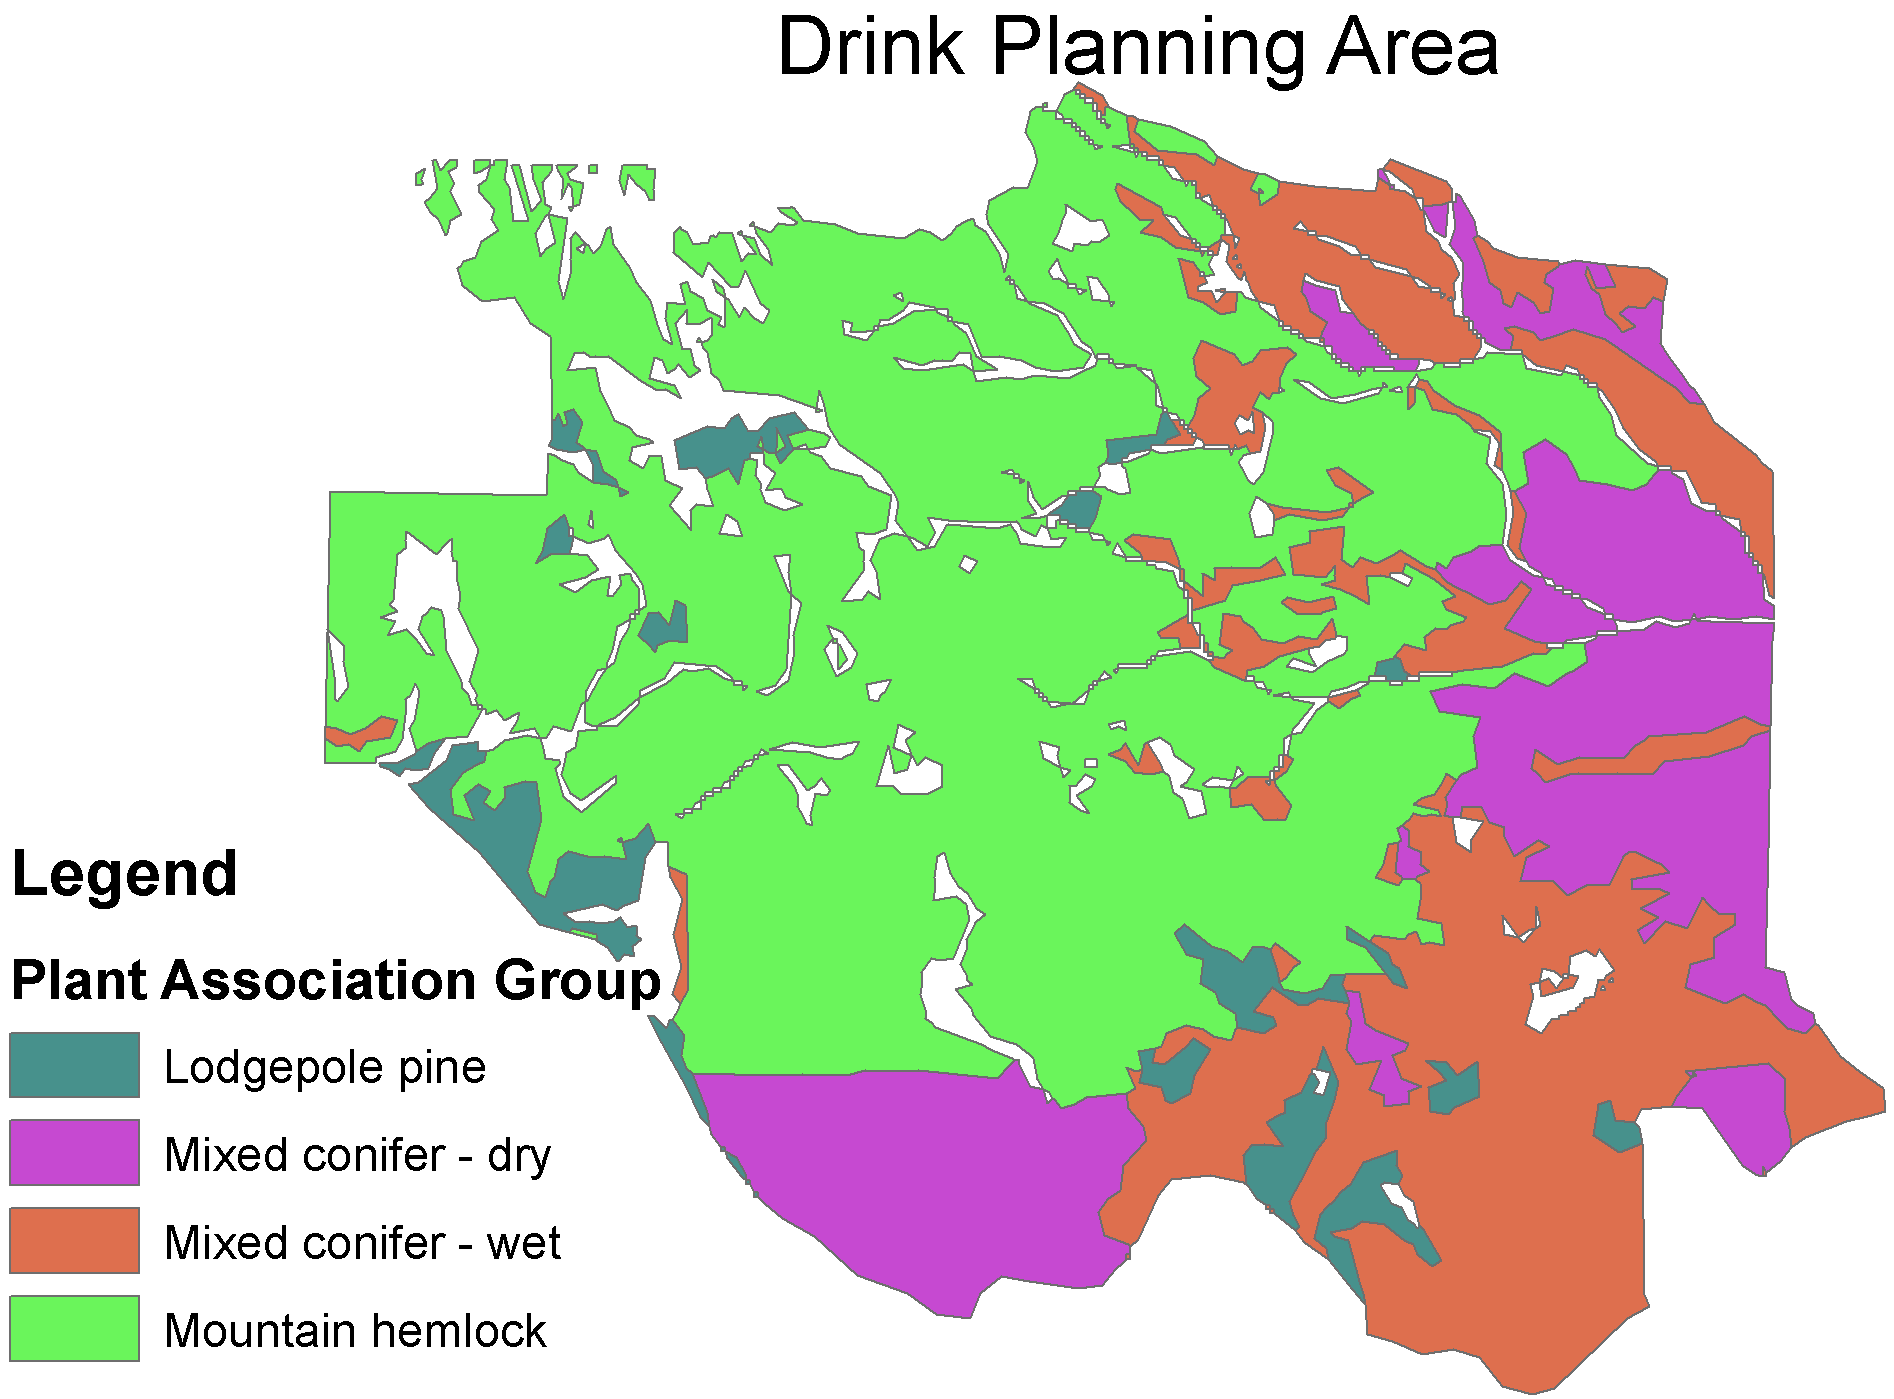
\includegraphics[width=.5\textwidth]{../images/DrinkMap_PAGs}
\caption[Plant association groups in the Drink Planning Area]{Plant association groups in the Drink Planning Area that were selected for potential treatments. Other plant association groups exist in the area but were not considered for treatment.}
\label{fig:drinkPAGs}
\end{figure}

The model minimizes the fire hazard rating of the Drink at the end of the 80-year planning horizon, maximizes the area of NSO habitat at the end of each planning period, and minimizes the short-term spikes in sediment delivery resulting from the application of silvicultural treatments.

Treatments are assumed to be performed at the midpoint year in the treatment period, years 2025 and 2045 for the first and second periods, respectively. A schematic of the planning horizon including the time of these events is shown in Figure \ref{fig:drinkPlanningHorizon}.

\begin{figure}
\centering
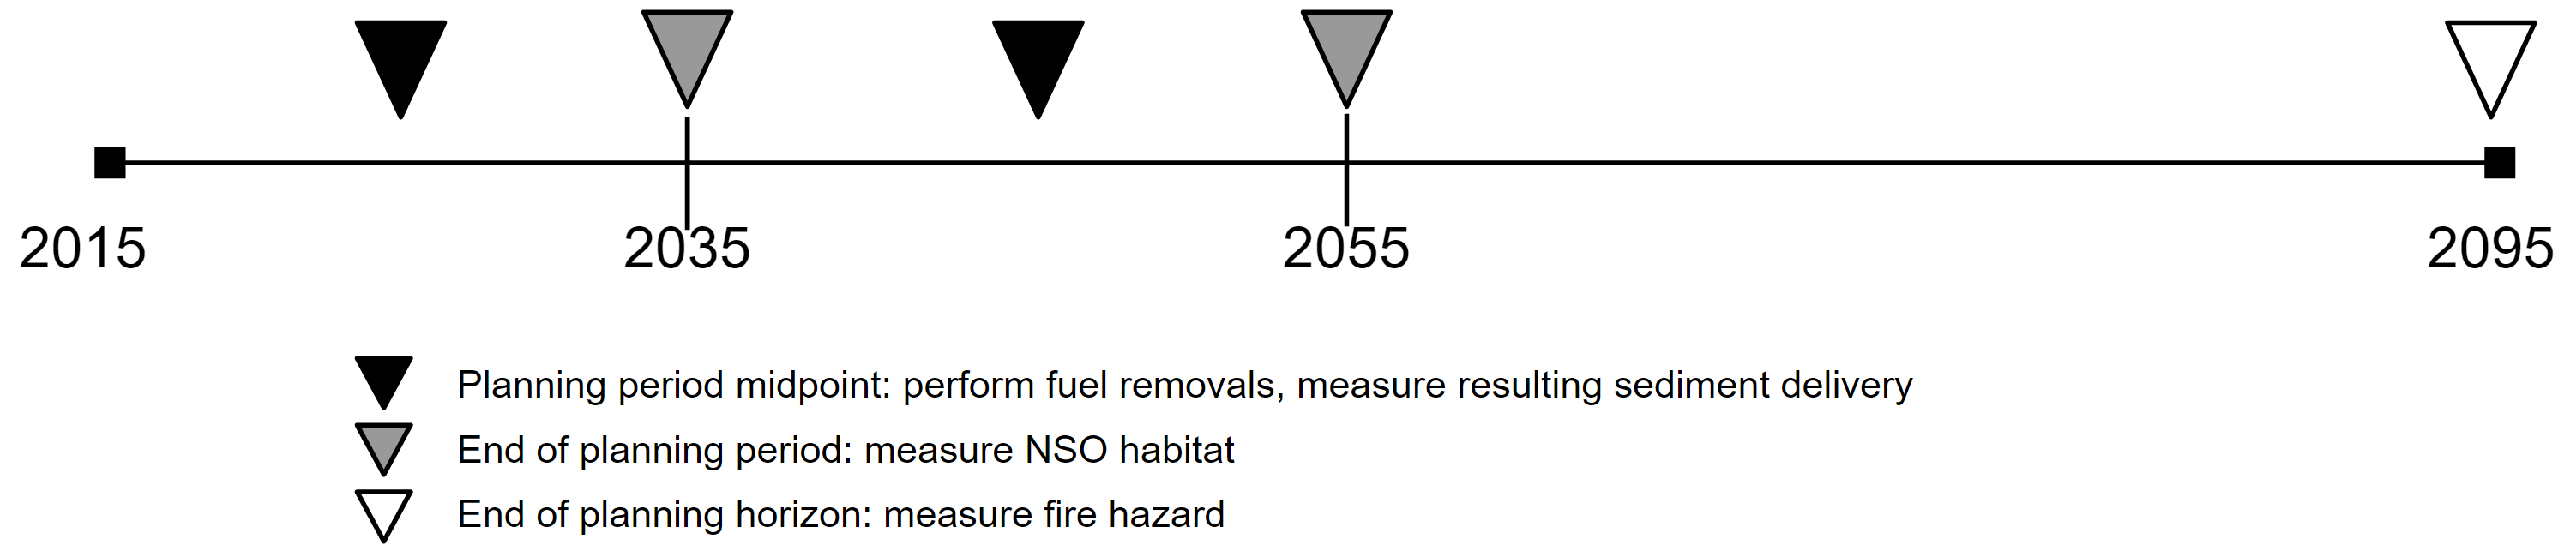
\includegraphics[width=.85\textwidth]{../images/Drink_PlanningHorizon_Sketch}
\caption[Planning horizon schematic]{The planning horizon used in the analysis spans the 80 year period from 2015 to 2095. Treatments may be performed in the first period, the second period, both, or neither. Treatments are assumed to be performed at the mid-point years of each period (black triangles). Sediment delivery is measured on treatment years. Stands' suitability for NSO habitat is measured at the end of the planning periods (gray triangles), and stands' fire hazard ratings are measured at the end of the planning horizon (white triangle).}
\label{fig:drinkPlanningHorizon}
\end{figure}

\subsubsection{Notation}
The following notation is used throughout the model:
\paragraph{Parameters}
\begin{itemize}
\item \textbf{$i \in I$:} the set of all 303 forest stands comprising the Drink area
\item \textbf{$r \in R$:} the set of treatment schedule prescriptions:
	$$
	r =
	\begin{cases}
	1 &\text{ treatment applied in the first period (2015-2035)}\\
	2 &\text{ treatment applied in the second period (2035-2055)}\\
	3 &\text{ treatment applied in both periods}\\
	0 &\text{ no treatment applied in either period}
	\end{cases}
	$$
\item \textbf{$F_{i,r}$:} the area-weighted fire hazard rating of stand $i$ at the end of the planning horizon if prescribed to treatment schedule $r$
\item \textbf{$I_{\omega,t}$:} the set of stands that can qualify as NSO habitat at the end of planning period $t$
\item \textbf{$a_i$:} the area of stand $i$
\item \textbf{$e$:} the discount factor applied to NSO habitat that is less than 200 ha in size
\item \textbf{$j \in R_{i,t}$:} the set of treatment schedules such that stand $i$ qualifies as NSO habitat in planning period $t$
\item \textbf{$s_{i,t}$:} the contribution in tons of sediment delivered from performing fuel treatments on stand $i$ in planning period $t$
\item \textbf{$c \in C$:} the set of all clusters of stands whose combined area exceeds 200 hectares
\item \textbf{$i \in D_c$:} the set of all stands that comprise cluster $c$
\item \textbf{$c \in C_i$:} the set of all clusters that contain stand $i$
\item \textbf{$A$:} the maximum area in hectares that may be treated in either planning period
\item \textbf{$\ell$, $u$:} the lower and upper bounds, respectively, on the relative fluctuation in the area treated in periods 1 and 2
\end{itemize}

\paragraph{Decision Variables}
$$
x_{i,r} = \begin{cases}
1 &\text{ if stand $i$ is prescribed to treatment schedule $r$}\\
0 &\text{ otherwise}
\end{cases}
$$ 

\paragraph{Indicator Variables}
\begin{itemize}
\item \textbf{$q_{c,t} = 1$} if all stands in cluster $c$ qualify as NSO habitat in planning period $t$ and $q_{c,t} = 0$ otherwise
\item \textbf{$p_{i,t} = 1$} if in planning period $t$ stand $i$ is part of a cluster $c$ such that $q_{c,t} = 1$; $p_{i,t} = 0$ otherwise
\end{itemize}

\paragraph{Accounting Variables}
\begin{itemize}
\item \textbf{$S_t$:} the contribution in tons of sediment delivered from performing fuel treatments in planning period $t$
\item \textbf{$O_t$:} the amount of NSO habitat in hectares at the end of planning period $t$
\item \textbf{$H_t$:} the area in hectares treated in planning period $t$
\end{itemize}

\subsubsection{Parameterization}
The model was parameterized as follows:
\begin{itemize}
\item \textbf{$F_{i,r}$:} the metric for fire hazard rating used in this analysis originated in the work by Schroder \textit{et al.} \cite{schroder2016multi}. This metric was developed for the Drink area. It uses fire characteristics from Anderson's fuel models \cite{anderson1982aids} to assign a fire hazard rating. I expanded the rating system to include fuel models not present in Schroder \textit{et al.} See Table \ref{tab:firehazards}.

The stands' fuels and vegetation characteristics to determine the fire hazard rating were generated using the US Forest Service's Climate-Forest Vegetation Simulator (FVS). Input vegetation data to Climate-FVS came from the 2012 GNN structure map (\url{http://lemma.forestry.oregonstate.edu/data/structure-maps}) from Oregon State University's Landscape Ecology, Modeling, Mapping \& Analysis (LEMMA) group. Plots from the LEMMA database were mapped to the stands in the Drink area in order to produce tree and stand lists. These lists were used with Climate-FVS to simulate the stands' vegetation and fuels characteristics forward for the duration of the planning horizon under each climate scenario. Input climate data for Climate-FVS was obtained through the Climate-FVS climate data server \cite{climateFVSReadyData}.
\item \textbf{$I_{\omega,t}$:} the set of stands that qualify as NSO habitat at the end of a planning period $t$ are those that meet the following three criteria, as specified by the USFS:
	\begin{enumerate}
	\item elevation less than 1830 m
	\item the presence of trees with DBH no less than 76 cm
	\item canopy closure of at least 60\%
	\end{enumerate}
The elevation requirement was checked using a digital elevation model from the US Department of Agriculture's GeoSpatial Data Gateway; canopy closure and large tree requirements were determined using the simulated vegetation characteristics output from Climate-FVS.

To account for the NSO's large habitat requirements, stands must also be members of a cluster exceeding 200 ha in size, the entirety of which meets the aforementioned NSO habitat criteria. Stands not part of such a cluster have their contributions to owl habitat discounted by a factor of $e$.
\item \textbf{$e$:} the discount factor for sub-200 ha NSO habitat was set to $e = 0.5$ following the convention used in Schroder \textit{et al.} \cite{schroder2016multi}.
\item \textbf{$j \in R_{i,t}$:} each stand-treatment schedule combination is evaluated at the end of each planning period to determine its suitability as NSO habitat. Treatment schedules for which stand $i$ meets the NSO habitat criteria at the end of treatment period $t$ become members of the set $R_{i,t}$. 
\item \textbf{$s_{i,t}$:} the contributions of sediment delivery from treatment of stand $i$ in period $t$ were determined using the Watershed Erosion Prediction Project (WEPP) online GIS tool \cite{frankenberger2011development}. This tool takes as input soil textures, treatment types, duration of simulation, and custom climate data. Soil texture data for the Drink area was obtained from the USDA's Soil Survey Geographic (SSURGO) database, treatment types are those specified in \S \ref{chap:appBTreatmentSpec}, and the years of simulation correspond to the treatment years in the model's planning horizon (2015-2095). The custom climate data are those described above for use with Climate-FVS, obtained through the Climate-FVS data server.
\item \textbf{$C$,$D_c$,$C_i$:} the formulation of clusters was performed \textit{a priori} according to the algorithm used in Rebain and McDill (2003) \cite{rebain2003mixed}. The enumerated clusters can then be used to immediately determine cluster members $D_c$ and cluster-stand relationships $C_i$.
\item \textbf{$A$:} the maximum area that may be treated in either planning period was defined to be 6000 acres, or approximately 2428 ha
\item \textbf{$\ell$, $u$:} the relative fluctuation in the area treated in periods 1 and 2 was defined to be 20\%. That is, the lower bound $\ell = 0.8$, and the upper bound $u = 1.2$.
\end{itemize}
\begin{table}[!ht]
\centering
\resizebox{\textwidth}{!}{%
\begin{tabular}{l|c|crrr}
\multicolumn{1}{c|}{Fuel Model} & \multicolumn{1}{c|}{\textbf{Fire Hazard Rating}} & \multicolumn{1}{c}{Group} & \multicolumn{1}{c}{Flame length (m)} & \multicolumn{1}{c}{Rate of spread (m/hr)} & \multicolumn{1}{c}{Total fuel load (tons/ha)} \\ \hline
4*                              & \textbf{5}                                       & Shrub                     & 5.79                                 & 1508.76                                   & 32.12                                         \\
5                               & \textbf{4}                                       & Shrub                     & 1.22                                 & 362.10                                    & 8.65                                          \\
8                               & \textbf{1}                                       & Timber                    & 0.30                                 & 32.19                                     & 12.36                                         \\
9*                              & \textbf{2}                                       & Timber                    & 0.79                                 & 150.88                                    & 8.65                                          \\
10                              & \textbf{2}                                       & Timber                    & 1.46                                 & 158.92                                    & 29.65                                         \\
11*                             & \textbf{2}                                       & Logging Slash             & 1.07                                 & 120.7                                     & 28.42                                         \\
12                              & \textbf{4}                                       & Logging Slash             & 2.44                                 & 261.52                                    & 85.50                                         \\
13                              & \textbf{5}                                       & Logging Slash             & 3.20                                 & 271.58                                    & 143.57                                       
\end{tabular}%
}
\caption[Fire hazard ratings used in multi-objective model]{Fire hazard rating system used here, originally employed by Schroder \textit{et al.} \cite{schroder2016multi}.\\
* denotes fuel models not present in Schroder \textit{et al.}\\
The fuel model column refers to the Anderson fuel model ratings \cite{anderson1982aids}.}
\label{tab:firehazards}
\end{table}

\subsubsection{Formulation}
The formulation of the model is as follows:
\begin{align}
Minimize \quad & \notag\\
&\sum_{i\in I}\sum_{r\in R} F_{i,r} x_{i,r} \label{eqn:objFire} \\
&\max \{S_1,S_2\} \label{eqn:objSediment} \\
Maximize \quad & \notag\\
&\min \{O_1,O_2\} \label{eqn:objOwl}
\end{align}
Subject to:
\begin{align}
\sum_{i\in I_{\omega,t}} \left(a_i p_{i,t} + e a_i \left( \sum_{j \in R_{i,t}} x_{i,j}-p_{i,t} \right) \right) &= O_t \qquad \forall t \in \{1,2\} \label{eqn:constraintDefOwl}\\
\sum_{i\in I} \sum_{r\in 1,3} s_{i,1} x_{i,r} &= S_1 \label{eqn:constraintSediment1} \\
\sum_{i\in I} \sum_{r\in 2,3} s_{i,2} x_{i,r} &= S_2 \label{eqn:constraintSediment2} \\
\sum_{i \in D_c} \sum_{j \in R_{i,t}} x_{i,j} - |c| q_{c,t} &\ge 0 \qquad \forall t \in \{1,2\}, c \in C \label{eqn:constraintClusterTriggers} \\
\sum_{c \in C_i} q_{c,t} - p_{i,t} &\ge 0 \qquad \forall t \in \{1,2\}, i \in I_{\omega,t} \label{eqn:constraintPVarTriggers} \\
\sum_{r \in R} x_{i,r} &= 1  \qquad \forall i \in I \label{eqn:constraintOnePrescrip} \\
\sum_{i \in I} \sum_{r \in 1,3} a_i x_{i,r} &= H_1 \label{eqn:constraintAreaAcctg1} \\
\sum_{i \in I} \sum_{r \in 2,3} a_i x_{i,r} &= H_2 \label{eqn:constraintAreaAcctg2} \\
H_t &\le A \qquad \forall t \in \{1,2\} \label{eqn:constraintAreaRestr} \\
\ell H_1 - H_2 &\le 0 \label{eqn:constraintAreaFlucL} \\
-u H_1 + H_2 &\le 0 \label{eqn:constraintAreaFlucU} \\
x_{i,r}, p_i, q_c \in \{0,1\} \quad &\forall i \in I, r \in R, c \in C \label{eqn:constraintNonNeg}
\end{align}

Equations \eqref{eqn:objFire}-\eqref{eqn:objOwl} are the objective functions: equation \eqref{eqn:objFire} minimizes the cumulative fire hazard rating of the Drink area at the end of the 80-year planning horizon, equation \eqref{eqn:objSediment} minimizes the maximum peak in sediment delivery for the two planning periods, and equation \eqref{eqn:objOwl} maximizes the minimum NSO habitat available at the end of the planning periods. Equation set \eqref{eqn:constraintDefOwl} defines the amount of NSO habitat available at the end of the planning horizons. Note that if stand $i$ does not belong to a cluster of NSO habitat exceeding 200 hectares, then its area contribution to total NSO habitat is discounted by a factor of $e$. Equations \eqref{eqn:constraintSediment1} and \eqref{eqn:constraintSediment2} define the sediment delivered in planning periods one and two, respectively.

Inequality set \eqref{eqn:constraintClusterTriggers} controls the value of the cluster variables $q_{c,t}$ indicating clusters meeting NSO habitat criteria in each of the planning periods. Inequality set \eqref{eqn:constraintPVarTriggers} controls the value of the $p_{i,t}$ variables indicating stands' inclusion in NSO habitat clusters.

The set of equalities \eqref{eqn:constraintOnePrescrip} enforces the logical constraint that each stand must be prescribed to exactly one treatment schedule. Equations \eqref{eqn:constraintAreaAcctg1} and \eqref{eqn:constraintAreaAcctg2} are accounting constraints for the total area treated in each planning period, and inequalities \eqref{eqn:constraintAreaRestr} ensure that this area does not exceed the predefined per-period maximum. Inequalities \eqref{eqn:constraintAreaFlucL} and \eqref{eqn:constraintAreaFlucU} bound the fluctuation in treated area between the planning periods. Finally, constraint \eqref{eqn:constraintNonNeg} defines the decision and indicator variables as binary.

\subsection{Model Solution and Comparing Efficient Frontiers}
I developed an implementation of T\'{o}th's Alpha-Delta algorithm \cite{TothThesis} to solve the models utilizing the IBM ILOG CPLEX optimization engine. For a problem with $N$ objectives, the Alpha-Delta algorithm finds the optimal set of solutions by iteratively slicing the $N$-dimensional objective space with a tilted $N-1$ dimensional plane. The algorithm was implemented using an alpha parameter of $\alpha = .01$ and delta parameters of $\delta_{Hab} = 1$ ha and $\delta_{Sed} = 2$ tons for the NSO habitat and sediment delivery objectives, respectively.

The solution to a bounded and non-degenerate multi-objective optimization problem with $N$ objectives is a set of objective vectors (also called ``solutions'') $\mathbf{z} \in Z$ where $\mathbf{z}=[z^1,\ldots,z^N]$. The set of solutions $Z$ is referred to as the Pareto-optimal frontier or efficient frontier or, simply, frontier. The solutions comprising an efficient frontier have the special relationship such that no component of a solution $\mathbf{z}^i$ can be improved upon without one of the other components $\mathbf{z}^j$ ($j \neq i$) degrading. This quality is known as Pareto efficiency. For example, this relationship in the current problem means that further reducing the value of fire hazard in a solution would result in either additional sediment delivery, a reduction of NSO habitat, or both.

Thus the efficient frontier provides information on the trade-off relationship that exists between ecosystem services. Parameterizing and solving the above model for each of the climate scenarios generates three frontiers: $Z_{\text{None}}$, $Z_{4.5}$, and $Z_{8.5}$ for the None, Ensemble RCP 4.5, and Ensemble RCP 8.5 scenarios, respectively. Since climate data alone differentiates the models and their resulting frontiers, comparing the frontiers reveals the impacts of climate on the trade-off relationships among the ecosystem services. However, no standardized procedure exists to compare frontiers.

One applicable metric to compare frontiers is the volume of the $N$-dimensional objective space bounded by the frontier, known as the hypervolume indicator. Together with S\'{a}ndor T\'{o}th, I devised an algorithm to compute the value of the hypervolume indicator any general $N$-dimensional frontier. The algorithm proceeds by sorting the solutions according to one objective, then iteratively adding them to the frontier, each time computing the additional volume enclosed by the solution. Details of the algorithm may be found in the appendix, \S \ref{chap:appAHypervolumeAlgo}.

We developed this algorithm independently and later discovered that researchers in the field of Evolutionary Multi-objective Optimization (EMO) have developed similar algorithms to compute the hypervolume indicator. In the present study, the hypervolume indicator is used as a measure of conflict among ecosystem services. Comparing hypervolume indicators across frontiers offers a quantification of the impact of climate change on trade-off relationships among ecosystem services. In EMO, the hypervolume indicator is used to assess the performance of stochastic multi-objective optimization algorithms. Hence, while the metric is the same, the algorithm to compute it and its application are entirely unique in this study.

Upon realization of the use of the hypervolume indicator in EMO, I discovered additional frontier comparison metrics used in this field and have adopted them for use here. These include the following indicators: the additive binary epsilon, binary hypervolume, unary distance, additive unary epsilon, and unary spacing. Information on these indicators can be found in the appendix, \S \ref{sec:emoMetrics}.

In addition to frontier-level comparisons that measure conflict between all ecosystem services simultaneously, it is also worthwhile to consider how climate change may impact the relationship between two specific ecosystem services within the frontier. Here, I use two methods to determine this: $1)$ the hypervolume indicator of the nondominated frontier points in a 2D projection, and $2)$ the Pearson correlation coefficient between objectives. Details on these methods may be found in the appendix, \S \ref{sec:withinFrontierMetrics}.